\documentclass[a4paper,oneside,12pt]{report}
\usepackage{styles/fbe_tez}
\usepackage[utf8x]{inputenc}
\renewcommand{\labelenumi}{(\roman{enumi})}
\usepackage{amsmath, amsthm, amssymb}
\usepackage[bottom]{footmisc}
\usepackage{cite}
\usepackage{url}
\usepackage{graphicx}
\usepackage{longtable}
\graphicspath{{figures/}}
\usepackage{multirow}
\usepackage{subfigure}
\usepackage{comment} % for multiline comment
\usepackage{tabularx} % better table formatting
\usepackage{array} % for column type customization
\usepackage{float} % for [H] placement on figures - not to wrap figures to the next page for the sake of optimized text flow. with this structure we are using in, figures are being replaced on the exact place as they are in the text flow.


\begin{document}

% ===============================
% INTRODUCTION
% ===============================
\chapter{Introduction}

When we started this research, we asked ourselves a simple question: why do "smart" cities often feel so disconnected from the people who actually live in them? We see technology everywhere (sensors in our buildings, digital twins of our cities, and massive data centers managing national infrastructure). But despite all this tech, there seems to be a missing link. The person in the wheelchair trying to navigate a steep ramp, or the community trying to report a water leak, often feels like an afterthought in these grand digital systems.

Our goal in this term paper is to explore how we can bridge this gap. We don't want to just build another technical system; we want to find a way to make these environments "inclusive" and "participatory." To achieve this, we conducted a systematic review of eight academic papers, one government project and six open-source code repositories, identifying a critical need for a "middle layer" that connects high-level social goals with low-level technical implementation.

In this report, we propose the "Multi-Scale Participatory Framework," a conceptual model that links three spatial scales (Building, City, National) through three vertical layers: Participation, Data, and Governance. We try to piece together a solution by looking at a lot of different research (from high-level theories about co-creation to very specific technical papers about coding compliance rules). What we found was that while the pieces of the puzzle exist, they aren't really talking to each other. Our proposed framework is our humble attempt to put those pieces together into something that might actually work.

% ===============================
% PROBLEM DEFINITION
% ===============================
\chapter{Problem Definition}

As we dug deeper into the literature, a clear problem started to emerge. It wasn't that we lack the technology; it's that the technology and the people are in two different worlds.

On one side, we have the visionaries like Sanders\cite{Sanders2008} and Wilson\cite{Wilson2015}. They tell us that for a design to be successful, users need to be partners. They warn us that if we treat people as passive subjects, we end up with "smart" homes that people actually hate living in. This made a lot of sense to us. But on the other side, we have the technical experts. Researchers like Dave\cite{Dave2018} and Liciotti\cite{Liciotti2020} are doing amazing work connecting BIM models to IoT sensors and using artificial intelligence to understand human activity. But their work is often very focused on the "how" (how to get the data, how to process it) and less on the "who."

We noticed a "silo" (Dave et al.\cite{Dave2018} uses this word) problem. The building experts are solving building problems. The urban planners are solving city problems. And the national infrastructure teams are dealing with their own massive networks. But a water leak doesn't care about these boundaries. It starts in a building, flows into the city network, and affects the national resource. Currently, these systems don't really talk to each other.

Furthermore, even when we have standards like IFC for buildings, they are often used just for geometry, not for the kind of rich, participatory data we care about. We realized that if we want a truly inclusive smart environment, we need to break down these silos. We need a way to connect the "participation" that Sanders talks about with the "technical implementation" that Dave builds, and we need to do it across all scales (from the room you're sitting in to the country you live in).

% ===============================
% LITERATURE REVIEW
% ===============================
\chapter{Literature Review}

To understand how to solve this, we looked at nine key papers (actually one of them is a government project (Ofwat's project\cite{ThamesWater2024})). We tried to group them not just by date, but by what they actually taught us.

\section{The "Why": Participation and User Needs}
Everything starts with the user. Sanders' research\cite{Sanders2008} was a real eye-opener for us. They argue that we need to move from "user-centered design" to "co-creation." It's not enough to just watch people; we have to invite them to the design table. This gave us the theoretical backbone for our project: users are experts in their own lives.

Then we read Wilson's research\cite{Wilson2015}, and it was a bit of a reality check. They analyzed smart homes and found that they often fail because they ignore the complex, messy reality of family life. They showed us that "smart" doesn't always mean "helpful." This reinforced our belief that technology needs to be flexible and sensitive to how people actually live.

\section{The "How": Technical Foundations}
Once we understood the human need, we looked for the technical tools. Dave\cite{Dave2018} provided a crucial piece of the puzzle. They showed us how to integrate BIM (Building Information Modeling) with IoT (Internet of Things). This is how we can make a static building model "alive" with real-time data. It's the bridge between the physical walls and the digital signals.

Liciotti\cite{Liciotti2020} took it a step further. They used unsupervised learning to detect activities in a smart home. What struck us here was the potential for the house to "understand" what's happening without needing invasive cameras everywhere. It suggests that we can have smarts without sacrificing privacy, which is a big concern for us.

\section{The "Scale": From Buildings to Nations}
But we can't just stay inside the house. Mendonça\cite{Mendonca2024} showed us a really cool way to automate rule checking using IDS (Information Delivery Specification). They used it to check if a building meets accessibility standards. We thought, "Wow, this is how we translate a human rule (like 'door must be wide') into something a computer can check automatically."

Then Zhou\cite{Zhou2024} zoomed out to the city level. They talked about the "Quadruple Helix" (bringing together government, industry, academia, and citizens). It made us realize that our framework needs to support this kind of broad collaboration.

Finally, we looked at the Ofwat's\cite{ThamesWater2024} project. This was different because it's a real-world, national-scale infrastructure project. They are using open data and graph databases to manage water networks. It showed us that this isn't just academic theory; big organizations are actually trying to solve these data integration problems right now.

\section{The "Gap": Recent Attempts and Challenges}
We also looked at some very recent work to see what's happening right now. Aavild\cite{Aavild2024} tackled the hardware problem. They showed that running everything on a single Raspberry Pi is a bad idea and proposed a distributed system. This is practical advice for us: don't overload the local controller.

Adreani\cite{Adreani2024} built a "Digital Twin" for a smart city. It's an impressive system, but we felt it was still a bit top-down. It gathers data from everywhere, but we wondered: where is the user in that massive dashboard? This confirmed to us that while the "Digital Twin" technology is maturing, the "Participatory" part is still lagging behind.

% ===============================
% PROPOSED CONCEPTUAL FRAMEWORK
% ===============================
\chapter{Proposed Conceptual Framework}

Based on all this reading, we tried to come up with a framework that ties it all together.

\section{The Multi-Scale Participatory Framework}
We call our proposed solution the "Multi-Scale Participatory Framework." It's an attempt to organize the mess of technologies and social theories we found into something that might actually work. The core idea is simple: we can't just stack technologies on top of each other; we have to weave them together with social goals.

We pictured this as a "Vertical Integration" model. Instead of just having a smart building that talks to a smart city, we have three distinct scales that are cut through by three shared layers.

\subsection{The Three Scales}
\begin{itemize}
    \item \textbf{Building Scale (Blue):} This is where people actually live. It's the home automation systems, the sensors in the walls, and the local interfaces.
    \item \textbf{City Scale (Orange):} This is the neighborhood or the town. It's where buildings connect to share data about energy, waste, or traffic.
    \item \textbf{National Scale (Purple):} This is the big picture. It's the infrastructure rules, the water networks (like in the Thames Water project), and the national safety standards.
\end{itemize}

\subsection{The Cross-Cutting Layers}
What makes our framework different is that we don't treat these scales as separate worlds. We propose three vertical layers that run through all of them:

\begin{itemize}
    \item \textbf{Participation Layer:} This is the most important part. Inspired by Sanders\cite{Sanders2008}, this layer ensures that at every scale, there is a way for people to give feedback. It's not just a suggestion box; it's a structural part of the system. At the building level, it might be a simple button to adjust the temperature. At the city level, it could be a digital town hall for voting on new parks.
    \item \textbf{Data Layer:} This is the plumbing. It uses the graph technologies and open standards we saw in the Ofwat project\cite{ThamesWater2024} to make sure data flows smoothly. We use "Brokers" and "RDF Stores" to translate the raw data from sensors into something meaningful that can be shared across the network.
    \item \textbf{Governance Layer:} This defines the rules. It includes the automated compliance checks from Mendonça's research\cite{Mendonca2024}. It ensures that the system is safe, fair, and follows the law, no matter which scale you're operating at.
\end{itemize}

\section{The Internal Agent: A Backup Brain}
One thing we worried about was: what if the internet goes down? Or what if the central server is too slow? That's why we added the concept of an \textbf{Internal Agent}.

This is a local "brain" that lives at the Building Scale. It doesn't need the cloud to make safety-critical decisions. If a fire alarm goes off, or a gas leak is detected, the Internal Agent acts immediately. It listens to the local sensors and follows the local rules. It only talks to the upper layers when it needs to share long-term data or get updates. We think this makes the system much more resilient and responsive.

\begin{figure}[H]
    \centering
    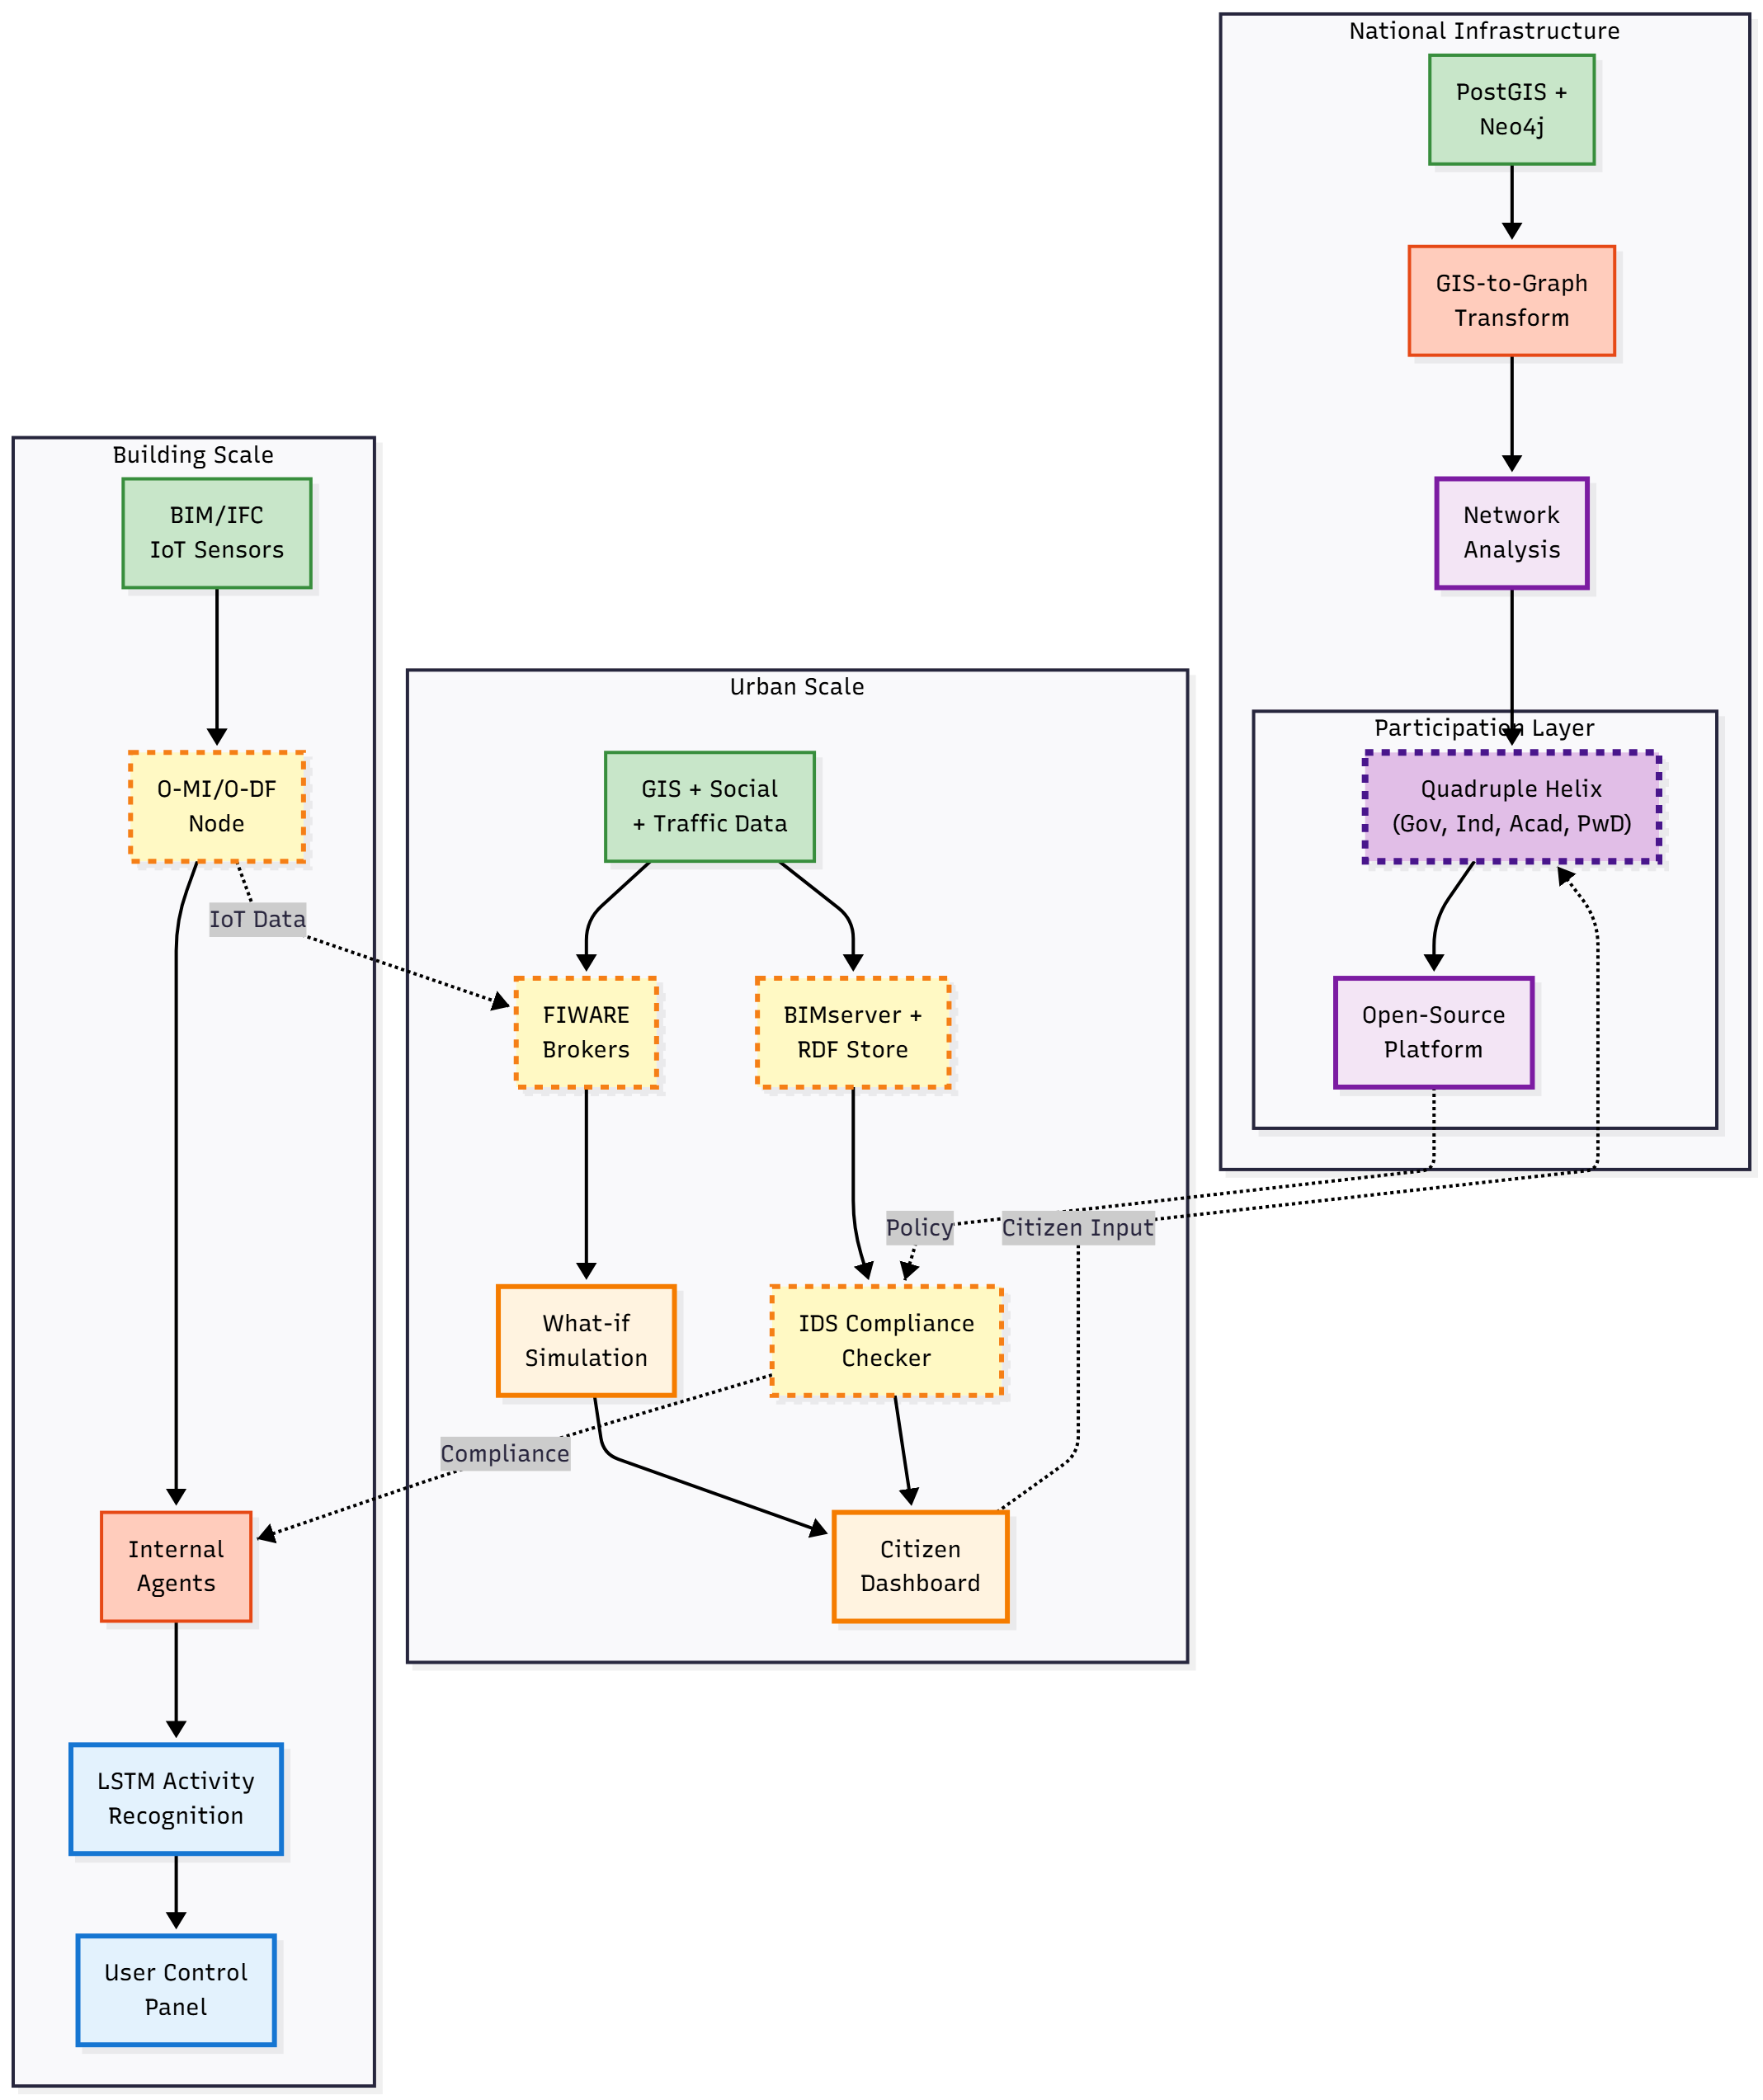
\includegraphics[width=\textwidth]{our-framework-proposal-vertical.png}
    \caption{Our proposed Inclusive Participatory Smart Environments Framework, showing the interaction between the three scales and the cross-cutting layers.}
    \label{fig:framework}
\end{figure}

We believe this structure gives us the best of both worlds: the efficiency of a connected smart city and the resilience and human-centric focus of a participatory home.

% ===============================
% DISCUSSION
% ===============================
\chapter{Discussion}

\section{Bridging the Gap: From Theory to Code}
One of the most striking things we found in our research was the disconnect between the "why" and the "how." Sanders and Stappers\cite{Sanders2008} gave us a beautiful vision of co-creation, where users are partners. But they didn't tell us how to code it. On the other hand, Dave et al.\cite{Dave2018} and Liciotti et al.\cite{Liciotti2020} gave us powerful tools for BIM and activity recognition, but they didn't really explain how these tools empower the average citizen.

\begin{figure}[H]
    \centering
    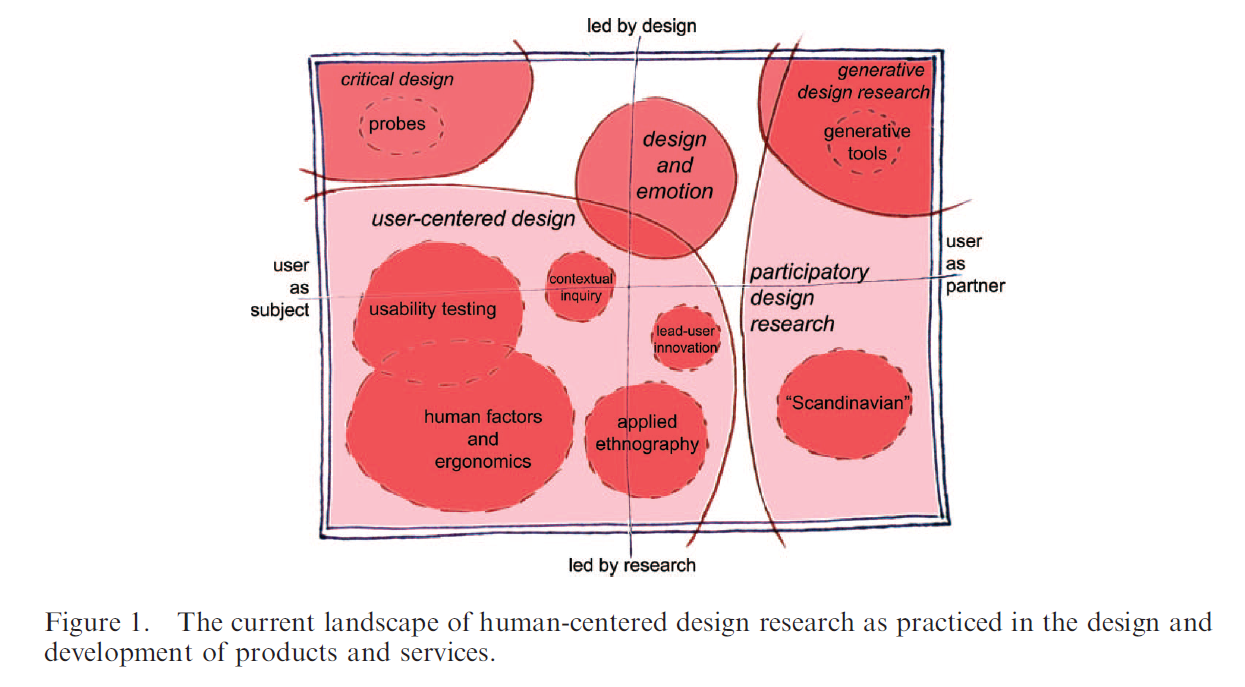
\includegraphics[width=0.8\textwidth]{sanders-participatory-framework.png}
    \caption{The shift from user-centered design to co-design, as visualized by Sanders and Stappers. We use this as the theoretical basis for our "Participation Layer."}
    \label{fig:sanders}
\end{figure}

Our "Multi-Scale Participatory Framework" is an attempt to bridge this gap. As shown in Figure \ref{fig:sanders}, the goal is to move users from being passive subjects to active co-creators. By placing the "Participation Layer" alongside the "Data" and "Governance" layers, we are arguing that user feedback is just as important as sensor data. It's not enough to just have a smart building that knows when to turn off the lights; we need a building that asks the user \textit{how} they want the lights to work.

\section{The Power of Vertical Integration}
We realized that the "silos" we talked about in the introduction aren't just horizontal (between different apps); they are vertical (between different scales). Aavild et al.\cite{Aavild2024} showed us how hard it is to run complex tasks on a single smart home device. But if we connect that home to the city scale, as suggested by the Snap4City project (Adreani et al.\cite{Adreani2024}), we can offload that processing.

\begin{figure}[H]
    \centering
    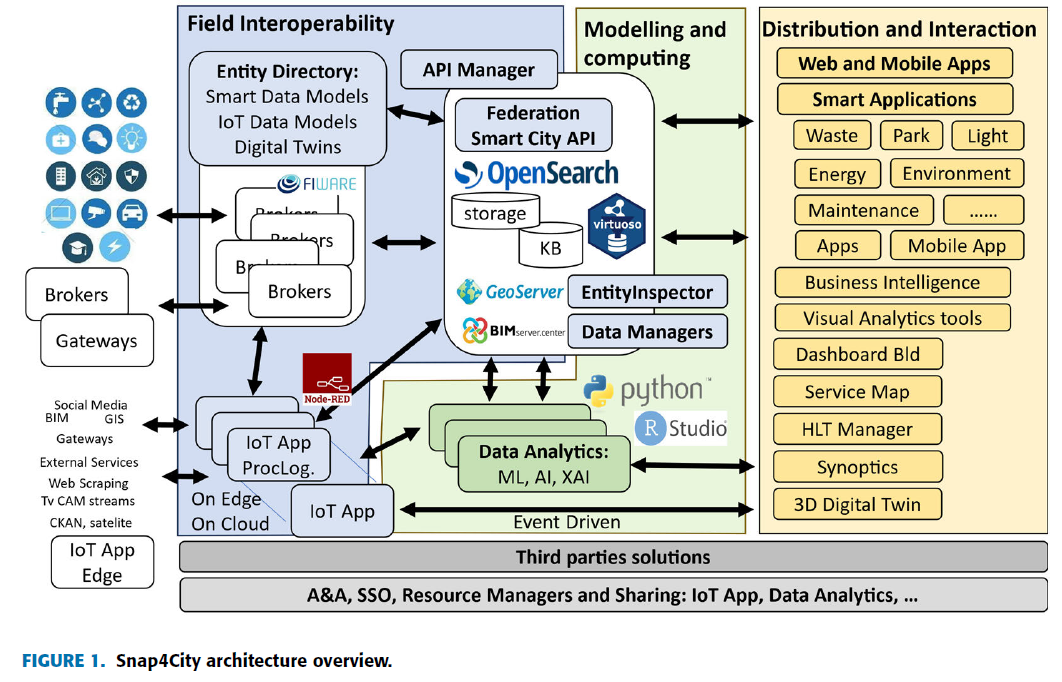
\includegraphics[width=0.9\textwidth]{adreani-snap4city-architecture.png}
    \caption{The complex architecture of a city-scale digital twin (Snap4City). Our framework aims to simplify or alter this by standardizing the vertical data flow.}
    \label{fig:adreani}
\end{figure}

This vertical integration, illustrated by the complexity of the Snap4City architecture in Figure \ref{fig:adreani}, also works for governance. The "National Scale" isn't just a distant bureaucracy; it's a library of rules (like the water network models from the Ofwat project\cite{ThamesWater2024}) that local systems can use. This means a small town doesn't have to invent its own water safety standards; it can just "download" them from the national layer.

\section{Technical Reality Check: A Code-Level Analysis}
To understand why this integration is so hard, we looked directly at the code in the repositories we analyzed. What we found was a clash of languages and logics that explains why these systems remain isolated.

\subsection{The Static World of IDS}
In the Mendonça and Ferreira repository\cite{Mendonca2024, MendoncaRepo}, the "rules" are written in XML. We analyzed the \texttt{IDS.xsd} schema and found that it relies heavily on \texttt{xs:restriction} to define simple limits (like "width > 1.2m"). But as we saw in their examples, this is purely static. It checks a file, not a living building. It has no concept of "time" or "state," which makes it very hard to use for real-time safety checks.

\begin{figure}[H]
    \centering
    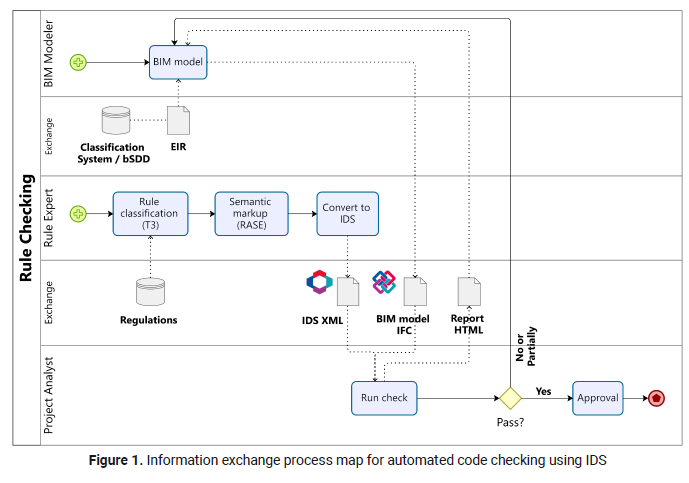
\includegraphics[width=0.9\textwidth]{mendonca-process.png}
    \caption{The automated compliance checking process using IDS. While efficient, it relies on static IFC files, creating a disconnect with real-time sensor data.}
    \label{fig:mendonca}
\end{figure}

As illustrated in Figure \ref{fig:mendonca}, the process is linear and file-based. You upload a model, check it, and get a report. There is no loop back to the user or the environment, which is a key limitation we identified.

\subsection{The Dynamic World of Snap4City}
In contrast, the Snap4City code (Adreani et al.\cite{Adreani2024, AdreaniRepo}) is all about real-time flow. We examined their \texttt{IoT Broker} component, which ingests JSON streams from thousands of sensors. Unlike the rigid XML of IDS, this data is messy and continuous. The \texttt{Data Inspector} script we looked at tries to clean this up, but it's a constant struggle against noise.

\subsection{The Distributed Logic of Home Assistant}
At the building scale, Aavild et al.\cite{Aavild2024, AavildRepo} tackle a different problem: hardware limits. Their \texttt{DistributionManager} class (which we analyzed in their Python code) dynamically offloads heavy tasks (like video processing) to other devices. This is brilliant for resilience, but it adds another layer of complexity. Now, a safety rule isn't just checking a value; it has to find a device to run the check on.

\begin{figure}[H]
    \centering
    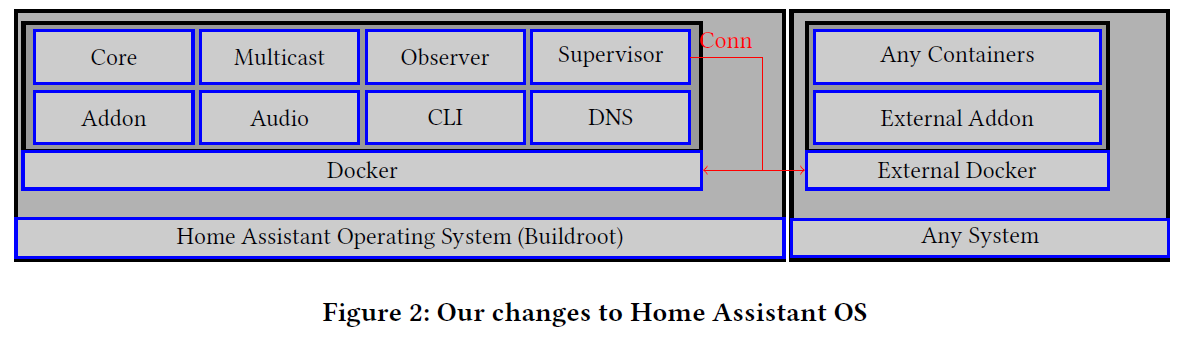
\includegraphics[width=0.9\textwidth]{aavild-external-devices.png}
    \caption{The distributed architecture proposed by Aavild et al., showing how heavy computational tasks are offloaded to external devices to prevent local hub saturation.}
    \label{fig:aavild}
\end{figure}

As shown in Figure \ref{fig:aavild}, this distributed approach ensures that a single point of failure (like an overloaded Raspberry Pi) doesn't crash the entire building's safety system. It's a critical piece of the "resilience" puzzle we're trying to solve.

\subsection{The National Ontology}
Finally, the Thames Water project\cite{ThamesWater2024, ThamesWaterRepo} uses a completely different approach: Ontologies. Their \texttt{Clean Water Module (CWM)} defines the network as a graph of nodes and edges. This is great for tracing a leak across a city, but it's totally incompatible with the \texttt{IFC} models used in buildings.

\subsection{The Integration Challenge}
So, we have XML for rules, JSON for sensors, Python classes for device management, and RDF graphs for national networks. Connecting these isn't just about plugging cables together; it's about translating between different ways of thinking. This is the core technical challenge our framework tries to address with the "Data Layer."

\section{Governance and the Quadruple Helix}
Finally, we have to talk about who runs all this. Zhou et al.\cite{Zhou2024} introduced us to the "Quadruple Helix" (the idea that Government, Industry, Academia, and Civil Society must work together).

\begin{figure}[H]
    \centering
    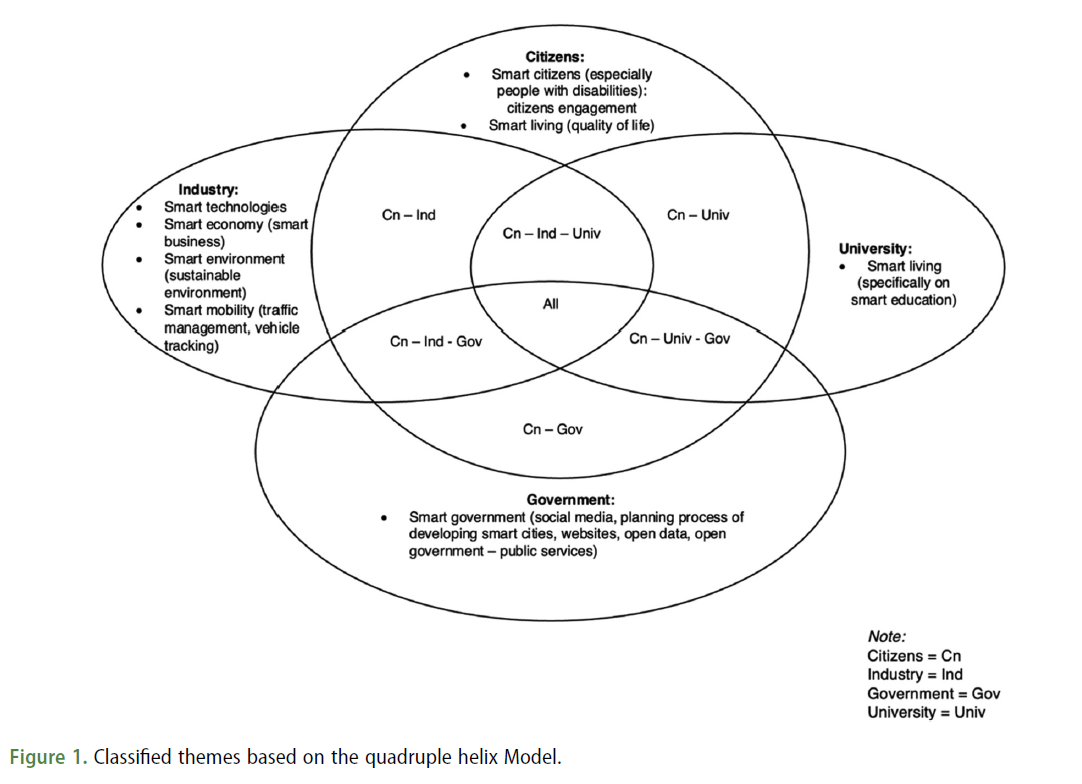
\includegraphics[width=1\textwidth]{zhou-quadruple-helix.png}
    \caption{The Quadruple Helix model of innovation. We adopted this to define the stakeholders in our "Governance Layer."}
    \label{fig:zhou}
\end{figure}

We think our framework supports this collaboration model (Figure \ref{fig:zhou}). The "Governance Layer" provides the rules (Government), the "Data Layer" provides the raw material for innovation (Industry and Academia), and the "Participation Layer" gives a voice to the people (Civil Society). Without all four, the system becomes unbalanced.

% ===============================
% CONCLUSION
% ===============================
\chapter{Conclusion}

\section{Summary of Findings}
In this term paper, we set out to find a way to make smart environments more inclusive. We started by looking at the problems: the silos, the lack of user voice, and the technical complexity. We then looked at the solutions offered by recent research, from distributed home automation to national water networks.

Our main contribution is the "Multi-Scale Participatory Framework." It's not a finished product, but a roadmap. It suggests that if we build our systems with participation, data, and governance as core, cross-cutting layers, we can create environments that adapt to people, rather than forcing people to adapt to them.

\section{Limitations}
We have to be honest about what we haven't done.
\begin{itemize}
    \item \textbf{Privacy vs. Utility:} As Liciotti et al.\cite{Liciotti2020} pointed out, tracking activities for safety is great, but it's also annoying. We haven't fully solved how to keep the "Participation Layer" from becoming a surveillance tool.
    \item \textbf{The Static-Dynamic Mismatch:} Our code analysis revealed a fundamental conflict. The safety rules (IDS) are static XML files, while the city data (Snap4City) is a dynamic JSON stream. Bridging this gap is not just a coding problem; it's a conceptual one.
    \item \textbf{Semantic Fragmentation:} We observed that different scales speak different languages. Buildings speak IFC, cities speak GIS, and national networks speak Graph/RDF. Currently, there is no universal translator between them.
    \item \textbf{Participation Fatigue:} Zhou et al.\cite{Zhou2024} warned us that if we ask people for feedback too often, they'll just stop caring. Our framework relies on active users, and if they burn out, the whole thing might fail.
    \item \textbf{Latency Risks:} Connecting a home to a national grid sounds cool, but if the internet cuts out, does the fire alarm still work? We tried to fix this with the "Internal Agent," but it's still a risk.
\end{itemize}

\section{Future Work}
Based on our findings, we see several promising directions for future research in this field:
\begin{itemize}
    \item \textbf{Automated Semantic Translation:} The biggest technical hurdle is the language barrier between scales. Future research should focus on developing "Automated Format Translators" that can automatically translate static XML rules into dynamic stream processors.
    \item \textbf{Prototyping the "Internal Agent":} A valuable next step would be to build a working prototype of the local "backup brain." Experiments could determine if low-cost hardware (like a Raspberry Pi) can effectively handle safety-critical logic during internet outages.
    \item \textbf{Piloting the "Participation Layer":} Theoretical models need real-world validation. Setting up a small-scale pilot (perhaps on a single floor of a building) would help researchers understand if and how residents actually engage with feedback tools.
    \item \textbf{Privacy-Preserving AI:} Exploring "Federated Learning" could offer a solution to the privacy concerns raised by Liciotti et al. In this model, AI learns on the device and only shares the \textit{lessons}, not personal data, which is a crucial area for further study.
    \item \textbf{Gamification Strategies:} To address the risk of "Participation Fatigue," future work could investigate how to make the feedback process more engaging. Mechanisms like rewards or "power discounts" might be effective in sustaining long-term user involvement.
\end{itemize}

We believe that the future of smart environments isn't just about smarter sensors; it's about smarter collaboration. And we hope our framework is a small step in that direction.


% ===============================
% REFERENCES
% ===============================
\bibliographystyle{styles/fbe_tez_v11}
\bibliography{references}
\end{document}
